\documentclass[7pt,a4paper]{article}

\usepackage{graphicx}
\usepackage{sectsty}

\sectionfont{\fontsize{10}{11}\selectfont}
\subsectionfont{\fontsize{10}{11}\selectfont}

\begin{document}
\textbf{\LARGE Assignment 2b Report - Text Mining}
\section{Introduction}
Given a collection of text documents we aim to find similar documents. In order to do that we normalized the text and created a Tf-idf matrix of collection and used cosine similarity to create a similarity matrix. Also applied K-means clustering and hierarchical clustering in order to identify clusters of similar documents.

\section{Packages Used - \textit{(Language: Python)}}
\begin{itemize}
\item{\textbf{Sklearn}:Package used for constructing Tf-idf, cosine similarity and for K-means}
\item{\textbf{NLTK}: Package used for Natural Language Processing.}
\item{\textbf{Scipy}: Package which provides function for plotting dendogram and linkage for Hierarchical Clustering.}
\item{\textbf{Seaborn}: Used for visualization of data through plots}
\item{\textbf{Matplotlib}: Used for plotting of graphs}
\item{\textbf{Pandas}: Package which provides Data structure like DataFrame which makes
manipulation of datasets easy}
\end{itemize}

\section{Dataset}
Twenty two text documents were taken all being on the Topic- \textbf{‘The History of web search engines’}. Texts are preprocessed and consists of terms corresponding to each document. 

\section{Methods and Observations}
\subsection{Tf-idf}
Stands for term frequency and inverse document frequency, is a numerical statistic that is intended to reflect how important a word is to a document in a collection.
Formula: tf-idf : tf * idf 
 				 
\subsection{K-means}
\begin{itemize}
\item{Used elbow method to find optimal numnber of clusters which came out of to be nine as the maximum drop in SSE error is at point nine as shown in the figure\ref{elbow}. Also, this has been verified using Silhoutte coefficient which also attains it's maximum value at iteration corresponding to nine clusters.}

\begin{figure}[h]
\centering
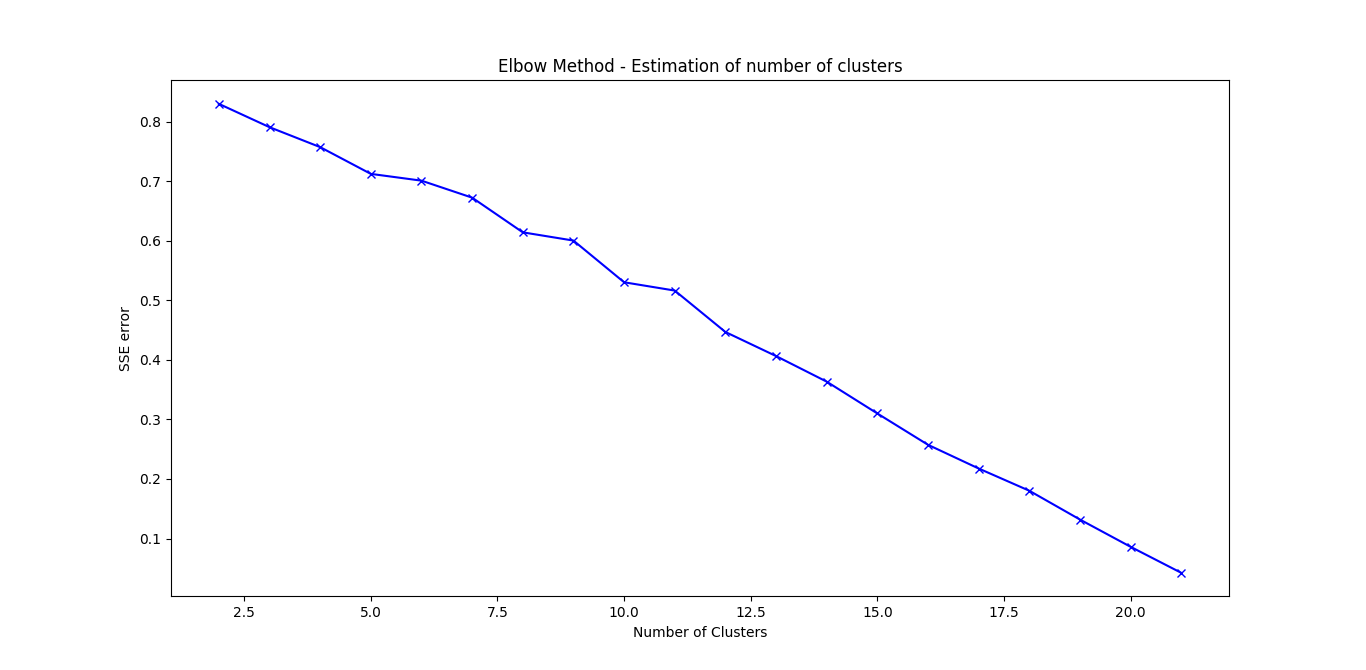
\includegraphics[scale=.40]{elbow}
\caption{Elbow method}
\label{elbow}
\end{figure}

\item{The clusters formed are as mentioned as follows:}
\begin{itemize}
\item{Cluster 0: \textit{Ass1-1147}}
\item{Cluster 1: \textit{Ass1-321}, \textit{Ass1-541}, \textit{Ass1-909}}
\item{Cluster 2: \textit{Ass1-1019}, \textit{Ass1-211},\textit{Ass1-505}, \textit{Ass1-532}}
\item{Cluster 3: \textit{Ass1-734}, \textit{Ass1-1037}, \textit{Ass1-743}}
\item{Cluster 4: \textit{Ass1-1349}, \textit{Ass1-936}, \textit{Ass1-826}}
\item{Cluster 5: \textit{Ass1-1046}, \textit{Ass1-1138}}
\item{Cluster 6: \textit{Ass1-422}, \textit{Ass1-440}}
\item{Cluster 7: \textit{Ass1-808}, \textit{Ass1-202}, \textit{Ass1-817}}
\item{Cluster 8: \textit{Ass1-606}}
\end{itemize}
\end{itemize}

\subsection{Cosine similarity}
\begin{itemize}
\item{It normalizes the lengths of the documents so smaller documents and longer documents have weights of the same order of magnitude.}
\item{According to the similarity matrix as shown in the figure, most similar documents comes out to be \textit{Ass1-422} and \textit{Ass1-440} (Similarity - 0.57) while the most dissimilar documents are \textit{Ass1-202} and \textit{Ass1-1046} (Similarity - 0.025)}
\textbf{Comparison with the previous Similarity matrix using Jaccard coefficient}
\begin{itemize}
\item{J.C. does not consider the frequencies of the terms in order to calculate the similarity between documents where as cosine similartity has been calculated using tf-idf vectors of the documents so the similarity between documents has increased as the term frequencies has been taken into account}
\end{itemize}
\end{itemize}
\begin{figure}[h]
\centering
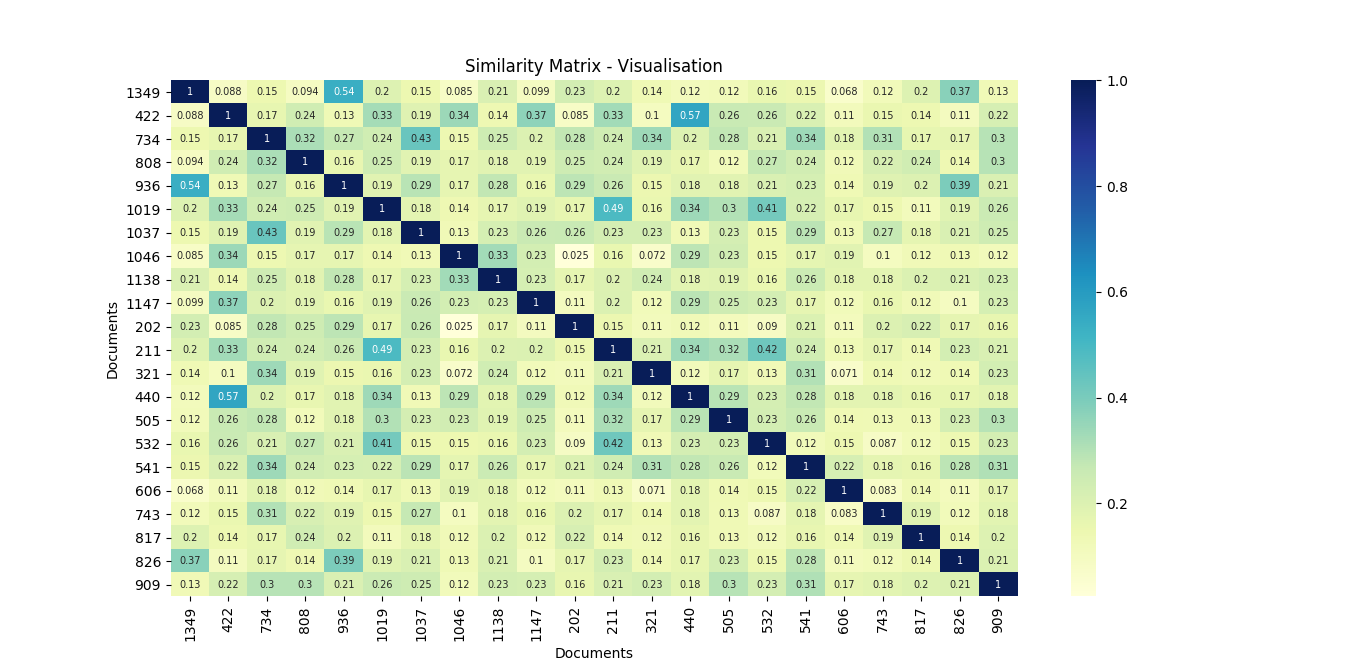
\includegraphics[scale=.40]{sim}
\caption{Similarity matrix - Cosine Similarity}
\label{image-Cos}
\end{figure}

\subsection{Hierarchical Clustering}
\begin{itemize}
\item{\textbf{Distance matrix}: It is obtained by calculating \textit{(1-Cosine Similarity)} between each pair of the documents as shown in the figure}
\item{\textbf{Linkage Parameter} : Single Linkage}
\item{Dendogram is shown in the figure \ref{image-Dendogram} below where the horizontal axis represents the pairwise dissimilarity between documents}

\begin{figure}[h]
\centering
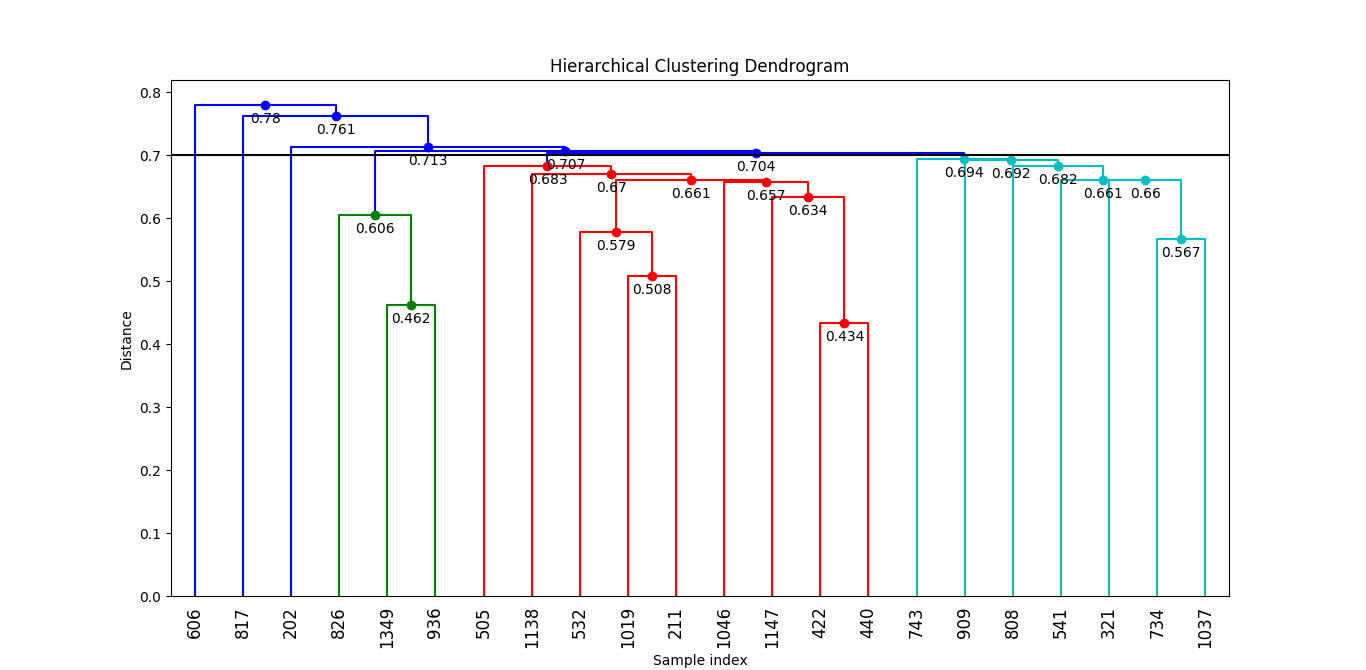
\includegraphics[scale=.40]{dendro}
\caption{Dendrogram}
\label{image-Dendogram}
\end{figure}

\item{}
\end{itemize}

\textbf{Comparison between K-means clustering and Hierarchical clustering}
\begin{itemize}
\item{K-means tries to minimise SSE by minimising the euclidean distance between the points belonging to the cluster and the center of the cluster.}
\item{In case of hierarchical clustering, cosine distance matrix has been used which is normalised so the different lengths may not neccessarily go into different clusters as in case of k-means clustering}
\begin{itemize}
\item{For instance, The documents \textit{Ass1-211} (Length - 359) \& \textit{Ass1-826} (Length - 240) }
\end{itemize}
\end{itemize}

\end{document}
